\section{Semantic analysis}

Checking that input program is well-typed, catching most errors. Generates typed AST. Strictly speaking, positions is no longer necessary for this part, but we would like to report errors with positions.\\

\textbf{Nominal type equivalence}: Two classes, although declared identically are not the same. Therefore, Arrays and Records in Tiger.light has a unique integer reference (\texttt{type unique = int ref}).\\

\textbf{Type environment}: Symbol map of name/identifier (\texttt{symbol} type in implementation) to type.\\

\textbf{Name type}: Necessary for mutual recursion in types (Records or arrays). Two traversals: Creating placeholder \texttt{name} types. Changing static link placeholder with correct type in second traversal.

\begin{figure}[h]
    \centering
    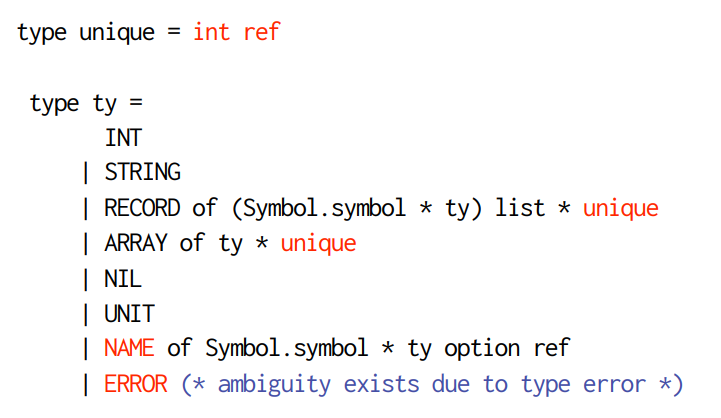
\includegraphics[scale=0.5]{assets/tigerlight_types.PNG}
    \caption{Tiger light types}
    \label{tiger_types}
\end{figure}

\textbf{Recusive functions}: Two traversals: First, collect function signatures (return and parameter types etc.) and add to environment. Second, for each function check that body matches declared signature.

